\documentclass[runningheads]{llncs}
%
\usepackage[T1]{fontenc}
\usepackage{graphicx}
\usepackage{amsmath, amssymb}
\usepackage{booktabs}
\usepackage{hyperref}
\usepackage{color}

% Custom configuration for hyperref
\hypersetup{
    colorlinks=true,
    linkcolor=blue,
    citecolor=blue,
    urlcolor=blue
}

\begin{document}
%
\title{LLM Agents for Interlinked and Personalised Knowledge Bases}
%
\titlerunning{LLM Agents for Personalised Knowledge Bases}
%
\author{Muhammed Furkan Kaya}
%
\authorrunning{M. F. Kaya}
%
\institute{Vrije Universiteit Amsterdam, Amsterdam, The Netherlands\\
\email{m.f.kaya@student.vu.nl}\\
\textbf{Supervisor:} Emile van Krieken \and
\textbf{Second Assessor:} Frank van Harmelen
}
%
\maketitle              % typeset the header of the contribution
%
\begin{abstract}
Personal Knowledge Management systems can help researchers organise
scientific literature as interconnected notes, but manually extracting
metadata, summarising papers, and maintaining links between related
documents requires substantial effort. This thesis evaluates a
multi-agent pipeline that transforms academic PDFs into structured,
interlinked Obsidian Markdown notes.

The system was evaluated on a personal research collection of 40
academic papers. Retrieval was compared across three configurations:
Flat RAG over raw PDF chunks, Structured RAG over agent-generated notes,
and Link-Expanded RAG, which additionally uses generated wiki-links
during ranking. The pipeline was also evaluated for bibliographic
metadata extraction, topic annotation, and citation-reference
extraction.

Structured notes did not consistently outperform chunk-based
retrieval, although they slightly improved the position of the first
relevant result. Link expansion achieved the highest observed
Recall@5, suggesting a modest benefit for retrieval coverage.
Bibliographic metadata extraction was generally accurate, with a
98\% title exact-match rate, whereas strict agreement with
expert-authored topic labels remained low. The Citation Link Agent
produced references with a precision of 0.84.

Overall, the pipeline was effective for automating bibliographic
organisation and generating reliable citation links. However, the
benefits of structured notes for retrieval were limited, and semantic
topic alignment remained sensitive to differences in vocabulary.


\keywords{Retrieval-Augmented Generation \and Personal Knowledge Graphs
\and Obsidian \and Multi-Agent Systems \and Information Retrieval}
\end{abstract}
%
%
%
\section{Introduction}
\label{sec:intro}

\subsection{Context and Motivation}

Conducting academic research requires continuously synthesising an expanding body of scientific literature. Discovering connections across papers, tracking research methodologies, and organising findings can impose a substantial cognitive burden. Personal Knowledge Management (PKM) systems such as Obsidian, Logseq, and Roam Research support this process by allowing users to organise information as interconnected notes.

Balog and Kenter define a Personal Knowledge Graph (PKG) as a resource containing structured information about entities that are personally related to its user~\cite{balog2019personal}. In this thesis, this concept is operationalised as a graph in which structured Markdown paper notes represent nodes and explicit Markdown wiki-links (\texttt{[[Note Target]]}) represent directed relationships between notes.

A well-maintained PKG can serve as an externalised research memory that reflects a researcher's individual understanding and organisational preferences. However, constructing and maintaining such a graph requires a substantial time investment to keep up with the vast volume of daily scholarly output. A researcher must manually obtain a paper, read it, extract bibliographic metadata, summarise its contributions, and identify relationships with previously stored literature. When this process is not maintained consistently, personal academic collections may devolve into folders of weakly connected PDFs and notes, reducing the potential benefits of graph-based organisation.

\subsection{Problem Statement}

Large Language Models (LLMs) offer a potential means of automating this ingestion process by extracting bibliographic metadata, generating structured summaries, and proposing links between related papers, thereby reducing manual management overhead. However, it remains unclear whether transforming raw academic documents into interlinked, agent-generated notes improves downstream Information Retrieval (IR) and provides useful support for researchers.

Retrieval-Augmented Generation (RAG) combines a generative language model with information retrieved from an external document collection~\cite{lewis2020retrieval}. In the Flat RAG baseline implemented in this thesis, raw PDF text is divided into sequential 512-token chunks with a 50-token overlap. Each chunk is embedded independently. For each query, a paper is assigned the similarity score of its highest-scoring chunk, after which the highest-ranked papers are returned. Although this approach is simple and computationally practical, it introduces two relevant limitations:

\begin{enumerate}
\item \textbf{Context Fragmentation:} A coherent argument, contribution, or methodological description may be divided across arbitrary chunk boundaries, causing retrieved units to contain incomplete context~\cite{sarthi2024raptor}.

\item \textbf{Loss of Inter-Document Context:} Independent vector retrieval does not explicitly incorporate graph structure or semantic relationships between papers during document ranking~\cite{edge2024local,gutierrez2024hipporag}.

\end{enumerate}

To investigate these limitations, this thesis implements a multi-agent ingestion pipeline that transforms academic PDFs into structured, Obsidian-compatible Markdown notes and generates typed semantic wiki-links between papers. Retrieval is evaluated using three configurations: Flat RAG over raw PDF chunks, Structured RAG over agent-generated notes, and Link-Expanded RAG, which applies an additional score boost to papers connected to the initially retrieved seed papers through the generated wiki-link graph. This design separates the effect of document restructuring from the additional effect of graph-informed link expansion.

\subsection{Research Questions and Hypotheses}
\label{sec:rqs}

The primary objective of this thesis is to determine whether transforming a flat PDF corpus into a network of structured, agent-generated notes improves retrieval within a personal academic knowledge base. Supporting research questions evaluate the extraction accuracy of metadata and bibliographic references, as well as the qualitative value of the generated notes.

\begin{quote}
\textit{To what extent can an LLM-agent ingestion pipeline improve retrieval in a personal knowledge base by generating structured notes and inter-note links, compared with a Flat RAG baseline?}
\end{quote}

This objective is addressed through four research questions and their corresponding hypotheses.

\subsubsection{RQ1: Retrieval Performance}

Does retrieval from structured, agent-generated Markdown notes, with or without graph-informed link expansion, improve search quality compared with retrieval from flat PDF chunks?

\begin{itemize}
\item[\textbf{H1:}] Structured RAG is expected to improve retrieval performance over Flat RAG by preserving paper-level context and reducing fragmentation. Link-Expanded RAG is further expected to improve retrieval by incorporating semantic relationships represented through inter-note wiki-links.
\end{itemize}

\subsubsection{RQ2: Metadata and Topic Extraction Accuracy}

How accurately can the LLM agent extract bibliographic metadata compared with reference records, and how well do its generated topic labels align with expert annotations?

\begin{itemize}
\item[\textbf{H2:}] Bibliographic metadata is expected to show higher agreement with reference records than generated topic labels show with expert-authored annotations.
\end{itemize}

\subsubsection{RQ3: Citation Reference Extraction Accuracy}

How accurately can an LLM-based Citation Link Agent extract explicit bibliographic references from academic papers compared with Semantic Scholar reference records?

\begin{itemize}
\item[\textbf{H3:}] The Citation Link Agent is expected to achieve
higher precision than recall because some bibliographic references may
be omitted during extraction.
\end{itemize}

\subsubsection{RQ4: Expert Evaluation of Generated Notes}

How does a domain expert assess the factual faithfulness, core-contribution coverage, structure and readability, and rediscovery utility of the agent-generated notes?

\begin{itemize}
\item[\textbf{H4:}] The agent-generated notes are expected to receive positive ratings from the domain expert, with average scores above the neutral midpoint across all evaluated dimensions.
\end{itemize}

% ============================================================

\section{Literature Study}
\label{sec:literature}

This section reviews research on retrieval in academic knowledge bases, agentic knowledge management and evaluation, and academic information extraction. These areas inform the design and evaluation of the proposed agent-generated personal knowledge base.

\subsection{Retrieval in Academic Knowledge Bases}

Retrieval-Augmented Generation (RAG) supplements language models with information retrieved from external text corpora~\cite{lewis2020retrieval}. A common baseline, Flat RAG, divides documents into fixed-size chunks, embeds each independently, and ranks documents based on the highest-scoring chunk similarity~\cite{qiu2024personal}. Although computationally practical, this introduces context fragmentation across chunk boundaries~\cite{sarthi2024raptor}. Structured RAG offers an alternative by representing each document through a single agent-generated summary containing bibliographic metadata, research goals, methods, and results.

Graph-based RAG methods incorporate semantic relationships between units to support multi-hop reasoning. Systems like GraphRAG detect communities and generate hierarchical summaries for global sensemaking~\cite{edge2024local}, while HippoRAG utilizes Personalized PageRank over concept graphs for associative retrieval~\cite{gutierrez2024hipporag}. While effective, full graph indexing introduces significant computational complexity. GraphRAG-Bench highlights the importance of evaluating graph construction and retrieval independently~\cite{xiao2025graphragbench}. This thesis evaluates a lightweight alternative: using Markdown wiki-links already stored in agent-generated notes to apply a one-hop score boost during document ranking.

\subsection{Agentic Knowledge Management and Evaluation}

Personal Knowledge Graphs (PKGs) organize information through personally meaningful relationships, where notes act as nodes and wiki-links encode directed edges~\cite{balog2019personal}. Agentic systems can automate this process by structuring, searching, and maintaining notes within personal databases like Obsidian~\cite{mybrainisfullcrew}. However, open-source implementations are rarely evaluated against external benchmarks or retrieval experiments.

Evaluating agent-generated notes requires human assessment, as automated metrics cannot determine factual reliability or utility. In summarization research, datasets like SummEval establish expert evaluation dimensions including consistency, relevance, coherence, and fluency~\cite{fabbri2021summeval}. This thesis adopts a similar exploratory expert evaluation covering factual faithfulness, core-contribution coverage, structure, and rediscovery utility to assess note quality.

\subsection{Academic Information and Citation Extraction}

Information extraction converts unstructured academic texts into structured metadata. LLM-based generative extraction prompts models to output structured fields (titles, authors, years, and references) directly from text~\cite{xu2024large}. Bibliographic extraction is generally objective, whereas topic tagging requires subjective interpretation, motivating separate evaluation protocols. Reference extraction (RQ3) specifically addresses recovering explicit bibliographies from paper text and comparing them to academic databases like the Semantic Scholar Academic Graph~\cite{kinney2023semantic}, which helps ground the system's external connectivity.

\subsection{Synthesis and Research Gap}

Existing work evaluates structured summaries, graph-based RAG, metadata extraction, and human summary quality in isolation. Graph RAG benchmarks typically focus on large corpora and global synthesis rather than personalized retrieval vaults. This thesis addresses this gap by evaluating a lightweight, Markdown-native ingestion pipeline across four aligned dimensions: retrieval performance, metadata extraction, citation extraction, and qualitative expert assessment.


% ============================================================
\section{Methodology}
\label{sec:methodology}

This section describes the academic-paper corpus, the multi-agent ingestion pipeline, the three retrieval configurations, and the evaluation procedures used to address RQ1--RQ4. The study combines quantitative evaluations of retrieval and extraction accuracy with an exploratory expert evaluation of the generated notes.

\subsection{Corpus and Data Preparation}
\label{sec:corpus}

The evaluation corpus consists of 40 academic papers selected from an existing personal research vault. The collection includes both published papers and preprints covering several areas relevant to the supervisor's research interests. Each paper is identified by its arXiv identifier and represented through three aligned artefacts: the original PDF, extracted plain text stored in JSON format, and an agent-generated Markdown note.

Before evaluation, automated preflight checks verified that the extracted texts, generated notes, queries, and relevance labels referred to the same 40 document identifiers. The generated notes were frozen before the experiments so that later citation-extraction processing could not modify the retrieval indexes or semantic links used in RQ1 and RQ2.

\subsection{Multi-Agent Ingestion Pipeline}
\label{sec:agent_pipeline}

The ingestion pipeline transforms raw academic papers into structured, Obsidian-compatible Markdown notes. Figure~\ref{fig:pipeline_diagram} illustrates the multi-agent architecture.

\begin{figure}[!htbp]
\centering
% \includegraphics[width=\textwidth]{pipeline_diagram.pdf}
\caption{Multi-agent ingestion pipeline architecture: PDF text is extracted and sequentially processed by the Metadata Agent, Summary Agent, and Semantic Link Agent to produce structured, interlinked Markdown notes in the local Obsidian vault.}
\label{fig:pipeline_diagram}
\end{figure}

The pipeline is organized into three sequential stages, operating as follows:

\begin{enumerate}
    \item \textbf{Metadata Extraction (Metadata Agent):} 
    \begin{itemize}
        \item \textit{Input:} The first two pages of the extracted paper plaintext.
        \item \textit{Model:} Google Gemini 2.5 Flash (default; configured with an automated fallback pool including OpenAI GPT-4o-mini if provider API quotas are exhausted).
        \item \textit{Output:} A structured JSON object containing bibliographic metadata (Title, Authors, Year, Venue, DOI, arXiv ID).
        \item \textit{Storage:} Written directly into the YAML frontmatter at the top of the generated Markdown file.
    \end{itemize}
    
    \item \textbf{Structured Note Generation (Summary Agent):}
    \begin{itemize}
        \item \textit{Input:} The entire plaintext of the paper PDF.
        \item \textit{Model:} Google Gemini 2.5 Flash.
        \item \textit{Output:} Structured summaries under five standardized sections: Overview/Summary, Methodology, Key Results, Limitations, and expert-assessment context.
        \item \textit{Storage:} Appended as Markdown text immediately below the YAML frontmatter of the note.
    \end{itemize}
    
    \item \textbf{Semantic Link Generation (Semantic Link Agent):}
    \begin{itemize}
        \item \textit{Input:} The current note and an index of all other paper titles and summaries in the database.
        \item \textit{Model:} Google Gemini 2.5 Flash.
        \item \textit{Output/Storage:} Generates typed, directional Markdown wiki-links (in the standard format \texttt{[[related\_paper\_title]]}) pointing to related works in the corpus, stored under a dedicated ``Related Papers'' section.
    \end{itemize}
\end{enumerate}

\paragraph{Citation Link Agent.}
A separate \textbf{Citation Link Agent} is used for RQ3. Rather than predicting conceptual semantic links, it processes the raw bibliography or references section of each paper. It extracts explicit bibliographic records and compares them against the Semantic Scholar API. If the cited work is present within the 40-paper corpus, it resolves it to a local wiki-link, bridging internal and external citation networks.

\paragraph{Automation and Parameters.}
Note creation, metadata parsing, and summarization are fully automated in a batch ingestion process. Semantic link and citation link extraction are triggered as separate, post-ingestion pipeline runs over the populated vault. Key retrieval parameters include a chunk size of 512 tokens, 50-token overlap, the 8192-token embedding model (\texttt{nomic-embed-text-v1.5}), and a top-$k = 5$ seed threshold for RAG retrieval.

\subsection{Retrieval Representations and Embedding Model}
\label{sec:retrieval_representations}

All three retrieval configurations use the SentenceTransformers framework~\cite{reimers2019sentence} with \texttt{nomic-ai/nomic-embed-text-v1.5}~\cite{nussbaum2024nomic}. Document and query embeddings are normalised, and similarity is calculated using cosine similarity.

The model-specific prefixes \texttt{search\_document:} and \texttt{search\_query:} are applied to documents and queries, respectively. The embedding model supports sequences of up to 8192 tokens, allowing each generated note to be represented as a single embedding.

\subsubsection{Flat RAG}
For the Flat RAG baseline, raw PDF text is tokenised using the embedding model's tokenizer and divided into sequential 512-token chunks with a 50-token overlap. Each chunk \(c_j\) belonging to paper \(d_i\) is embedded independently.

Paper-level ranking uses MaxP aggregation~\cite{dai2019deeper}. The score assigned to a paper is the highest cosine similarity obtained by any of its chunks:
\[
\operatorname{Score}_{\mathrm{Flat}}(d_i,q)
=
\max_{c_j \in d_i}
\cos\left(E(q),E(c_j)\right),
\]
where \(E(\cdot)\) denotes the embedding function. Papers are ranked in descending order of this maximum chunk score.

\subsubsection{Structured RAG}
For Structured RAG, each complete agent-generated Markdown note \(n_i\) is embedded as one paper-level retrieval unit:
\[
\operatorname{Score}_{\mathrm{Struct}}(d_i,q)
=
\cos\left(E(q),E(n_i)\right).
\]
To isolate the effect of document restructuring from graph information, paper-to-paper wiki-links are removed from the note text before embedding. Wiki-links referring to general topics or concepts are converted to plain text rather than removed.

\subsubsection{Link-Expanded RAG}
Link-Expanded RAG begins with the Structured RAG similarity scores. For each query \(q\), the five highest-ranked structured notes form the seed set \(S_q\). The system then reads the outbound wiki-links stored in those seed notes and identifies linked papers that are present in the corpus but not already part of the seed set.

Let \(N^{+}(S_q)\) denote the union of the outbound paper neighbours of the seed notes. The expanded score is:
\[
\operatorname{Score}_{\mathrm{Expanded}}^{(f)}(d_i,q)
=
\operatorname{Score}_{\mathrm{Struct}}(d_i,q)
+
\alpha_f
\mathbb{I}\left(d_i \in N^{+}(S_q)\right),
\]
where \(\mathbb{I}(\cdot)\) is the indicator function and \(\alpha_f\) is the link-boosting coefficient selected for cross-validation fold \(f\).

The coefficient was not fixed in advance. A five-fold stratified cross-validation procedure was used, with query categories preserved across folds. Candidate values were derived from similarity-score transitions between seed and linked papers. Within each fold, \(\alpha_f\) was selected using the training queries, prioritising MRR@5, followed by Recall@5, Precision@5, and finally the smallest coefficient in the event of a tie. Performance was then measured on the held-out queries.

\subsection{RQ1: Retrieval Evaluation}
\label{sec:rq1_method}

RQ1 evaluates Flat RAG, Structured RAG, and Link-Expanded RAG using 40 queries. The queries cover simple factual retrieval, comparisons between papers, and questions concerning neuro-symbolic methods. Each query is associated with one or more manually curated relevant papers.

The top five retrieved papers are evaluated using:
\begin{itemize}
    \item \textbf{Precision@5}, the proportion of the five retrieved papers that are relevant;
    \item \textbf{Recall@5}, the proportion of relevant papers retrieved within the first five positions; and
    \item \textbf{MRR@5}, the reciprocal rank of the first relevant paper, or zero when no relevant paper occurs in the top five.
\end{itemize}
Metrics are computed per query and macro-averaged across all 40 queries. The primary Link-Expanded RAG results use the aggregated held-out predictions from the five cross-validation folds.

\subsection{RQ2: Metadata and Topic Evaluation}
\label{sec:rq2_method}

RQ2 contains two evaluation groups. The bibliographic evaluation covers all 40 generated notes. Agent-extracted bibliographic metadata are compared with externally curated Semantic Scholar records.

Titles and publication years are evaluated using normalised exact matches. Venue matching combines text normalisation, known venue synonyms, acronym matching, and token-level Jaccard similarity. Author lists are treated as sets and evaluated using Precision, Recall, and F1.

The semantic evaluation covers the 22 papers that overlap with the supervisor's existing vault. The agent-generated \texttt{hasTopic} labels are compared with expert-authored topic annotations using set-based Precision, Recall, and F1. Paper titles incorrectly stored among the expert topic labels are removed before scoring. OpenAlex topics and keywords are used only as a supplementary check for agent-generated labels that are absent from the expert annotations.

\subsection{RQ3: Citation Reference Evaluation}
\label{sec:rq3_method}

RQ3 evaluates the extraction accuracy of bibliographic references under a single-variable controlled experiment. The controlled variable is \textbf{Input Coverage}, designed to assess the impact of input truncation on reference extraction performance:

\begin{enumerate}
    \item \textbf{Truncated Input (Baseline):} The system detects the References section of a paper PDF and truncates the text to the first 12,000 characters before sending it to the Citation Link Agent.
    \item \textbf{Complete Bibliography (Untruncated):} The system processes the complete References section text without any character truncation limits.
\end{enumerate}

To implement the untruncated pipeline while respecting model limits and API behaviors, the following architectural controls were introduced:
\begin{itemize}
    \item \textbf{Local Segmentation and Batching:} Long reference sections are split locally into individual citation strings using standard index markers. Citations are grouped into batches of 30 references per request. This prevents token timeouts, respects the provider's rate limits, and isolates copyrighted text blocks.
    \item \textbf{Recitation Block Handling:} To bypass Gemini's copyright filters (where the API blocks responses with \texttt{finish\_reason = RECITATION}), the pipeline detects recitation failures instantly. Instead of retrying, it bypasses the LLM for that specific batch and falls back to a local heuristic-based regex parser to extract candidate titles, protecting the overall recall of the pipeline.
\end{itemize}

All other experimental variables remain unchanged: the Citation Link Agent's prompt, the default model (Gemini 2.5 Flash), temperature (0.0), JSON schema, deduplication logic, matching hierarchy, 34-paper evaluation subset, and gold reference records.

Predicted and gold references are deduplicated using Semantic Scholar identifiers, DOIs, arXiv identifiers, and normalised exact titles. Matching is performed one-to-one in the following order: Semantic Scholar identifier, DOI, arXiv identifier, and normalised exact title. Once a gold record is matched, it cannot be matched again. Precision, Recall, and F1 are calculated from the aggregated true-positive, false-positive, and false-negative counts.

\subsection{RQ4: Qualitative Expert Evaluation}
\label{sec:rq4_method}

Because of the small sample size (five papers evaluated by a single domain expert), the human evaluation for RQ4 is designed as an exploratory, qualitative assessment rather than a statistically representative user study. It serves to identify usability patterns, model errors, and structural strengths of the agent-generated notes. For each of the five randomly sampled papers (selected using a pre-recorded random seed for reproducibility), the evaluator receives the paper title, abstract, source PDF, and the generated Markdown note.

The evaluator rates each note on a five-point Likert scale (1 = Poor, 5 = Excellent) across four key quality dimensions:
\begin{enumerate}
    \item \textbf{Factual faithfulness:} Extent to which the summary is free of hallucinations or factual errors.
    \item \textbf{Core-contribution coverage:} Completeness in capturing the main research contributions, datasets, and methods.
    \item \textbf{Structure and readability:} The stylistic flow, text organization, and presentation.
    \item \textbf{Utility for rediscovery:} The subjective value of the note as a memory aid in a personal knowledge base.
\end{enumerate}
Individual ratings, mean scores for each dimension, and qualitative feedback are recorded and summarized. The evaluation criteria are adapted from standard summarization frameworks~\cite{fabbri2021summeval}.


\subsection{Reproducibility and Experimental Controls}
\label{sec:reproducibility}

Corpus-alignment assertions ensure that the same document identifiers are used throughout the experiments. Embeddings and LLM predictions are cached to avoid unnecessary recomputation. The RQ3 prediction cache records the model name, temperature, prompt version, generation timestamp, and a hash of the Citation Link Agent source code. RQ1 and RQ2 artefacts remain frozen during RQ3, preventing later processing from altering the earlier experimental conditions.

\section{Results}
\label{sec:results}

This section presents the quantitative results for retrieval performance (RQ1), metadata and topic extraction accuracy (RQ2), citation-reference extraction accuracy (RQ3), and the qualitative expert evaluation (RQ4).

\subsection{RQ1: Retrieval Performance}
\label{sec:rq1_results}

Flat RAG and Structured RAG were evaluated across all 40 queries. Link-Expanded RAG reports the aggregated held-out predictions obtained through five-fold cross-validation. Table~\ref{tab:rq1_results} presents the macro-averaged retrieval metrics.

\begin{table}[!htbp]
\centering
\caption{Retrieval performance across the three configurations.}
\label{tab:rq1_results}
\begin{tabular}{lccc}
\toprule
\textbf{Configuration} & \textbf{Recall@5} & \textbf{Precision@5} & \textbf{MRR@5} \\
\midrule
Flat RAG & 0.70 & \textbf{0.24} & 0.73 \\
Structured RAG & 0.70 & 0.23 & \textbf{0.74} \\
Link-Expanded RAG & \textbf{0.72} & 0.23 & 0.74 \\
\bottomrule
\end{tabular}
\end{table}

Structured RAG achieved the same Recall@5 as Flat RAG. Its Precision@5 decreased from 0.24 to 0.23, while MRR@5 increased from 0.73 to 0.74. This indicates that the first relevant paper tended to occur slightly earlier in the ranking, although retrieval coverage did not increase.

Link-Expanded RAG achieved the highest Recall@5 at 0.72, an absolute increase of 0.02 over both Flat and Structured RAG. Its Precision@5 was 0.23, while its MRR@5 of 0.74 was nearly identical to the Structured RAG result. A visual comparison of these retrieval metrics is presented in Figure~\ref{fig:retrieval_metrics}.

\begin{figure}[!htbp]
\centering
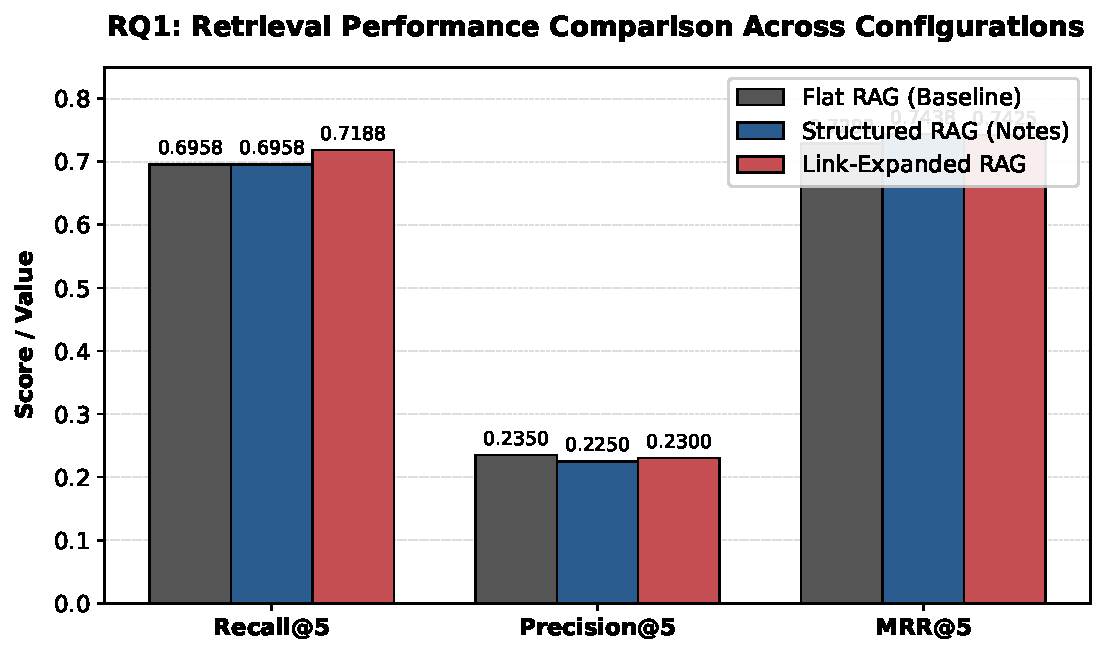
\includegraphics[width=0.9\textwidth]{retrieval_metrics.pdf}
\caption{RQ1: Retrieval performance comparison (Recall@5, Precision@5, and MRR@5) across Flat RAG (baseline), Structured RAG, and Link-Expanded RAG configurations.}
\label{fig:retrieval_metrics}
\end{figure}

\subsection{RQ2: Metadata and Topic Evaluation}
\label{sec:rq2_results}

RQ2 contains two evaluations. Bibliographic metadata were evaluated over all 40 papers, while semantic topic labels were evaluated over the 22 papers that overlapped with the expert-authored vault.

\subsubsection{Bibliographic Metadata}
Table~\ref{tab:rq2_group_a} reports the comparison between the agent-extracted bibliographic fields and the Semantic Scholar records.

\begin{table}[!htbp]
\centering
\caption{Bibliographic metadata extraction results.}
\label{tab:rq2_group_a}
\begin{tabular}{lc}
\toprule
\textbf{Metadata field} & \textbf{Score} \\
\midrule
Title exact match & 0.98 \\
Year exact match & 0.78 \\
Venue fuzzy match & 0.50 \\
Author-set F1 & 0.83 \\
\bottomrule
\end{tabular}
\end{table}

The highest result was obtained for title extraction, with an exact match rate of 0.98. Author extraction achieved an F1-score of 0.83, based on a precision of 0.82 and recall of 0.83. The year exact-match rate was 0.78, while venue matching produced the lowest bibliographic score at 0.50.

\subsubsection{Semantic Topic Labels}
The agent-generated \texttt{hasTopic} labels were compared with the expert-authored annotations using strict normalised set matching over the 22 overlapping papers. This evaluation produced a macro-averaged precision of 0.08, recall of 0.15, and F1-score of 0.10.

\subsection{RQ3: Citation Reference Evaluation}
\label{sec:rq3_results}

The Citation Link Agent was evaluated under both input coverage configurations against the outgoing reference lists obtained from the Semantic Scholar Academic Graph. Table~\ref{tab:rq3_results} presents the comparative evaluation metrics.

\begin{table}[!htbp]
\centering
\caption{Citation-reference extraction performance: Truncated (Baseline) vs. Complete Bibliography.}
\label{tab:rq3_results}
\begin{tabular}{lccccccc}
\toprule
\textbf{Configuration} & \textbf{Papers} & \textbf{TP} & \textbf{FP} & \textbf{FN} & \textbf{Precision} & \textbf{Recall} & \textbf{F1-score} \\
\midrule
Truncated Baseline & 34 & 1,060 & 197 & 863 & \textbf{0.8433} & 0.5512 & 0.6667 \\
Complete Bibliography & 37 & \textbf{1,514} & 283 & \textbf{534} & 0.8425 & \textbf{0.7393} & \textbf{0.7875} \\
\bottomrule
\end{tabular}
\end{table}

The results show that removing the 12,000-character truncation limit and processing the complete bibliography significantly improved extraction quality. Recall increased from 0.5512 to 0.7393 (an absolute improvement of +0.1881, or +18.8\%), which drove the F1-score up from 0.6667 to 0.7875 (+12.1\% absolute increase). Importantly, this substantial increase in coverage was achieved with virtually no loss in precision, which remained constant (0.8433 vs. 0.8425). 

This behavior supports Hypothesis H3: the agent maintains high precision, but its recall was previously bottlenecked by character truncation. By analyzing the entire bibliography, the total number of True Positives increased from 1,060 to 1,514, and False Negatives fell from 863 to 534.

Among the 1,514 true-positive matches in the untruncated configuration, 107 were resolved through DOI identifiers, 463 through arXiv identifiers, and 944 through normalised exact-title matches. No matches were established directly through a Semantic Scholar paper identifier, and no malformed predictions lacking all usable identifiers were included. Due to the integration of the local fallback parser, three papers that were previously excluded due to provider API blocks were successfully processed, increasing the scored papers count from 34 to 37.

\subsection{RQ4: Qualitative Expert Evaluation}
\label{sec:rq4_results}

The qualitative expert evaluation assessed the agent-generated notes across five randomly selected papers. Table~\ref{tab:rq4_results} shows the individual paper scores and dimension averages on the 1--5 Likert scale.

\begin{table}[!htbp]
\centering
\caption{Expert evaluation ratings (1--5 Likert scale) for the five randomly sampled papers.}
\label{tab:rq4_results}
\begin{tabular}{lccccc}
\toprule
\textbf{Paper ID} & \textbf{Title} & \textbf{Faithfulness} & \textbf{Coverage} & \textbf{Readability} & \textbf{Utility} \\
\midrule
2305.19951 & Not All Neuro-Symbolic... & 4 & 3 & 4 & 4 \\
2005.11401 & Retrieval-Augmented Gen... & 4 & 3 & 4 & 3 \\
2402.12240 & bears MAKE NEURO-SYMBOLIC... & 4 & 3 & 3 & 3 \\
2401.15884 & Corrective Retrieval... & 3 & 2 & 3 & 2 \\
2401.05224 & Do Vision and Language... & 4 & 4 & 3 & 4 \\
\midrule
\textbf{Mean} & & \textbf{3.80} & \textbf{3.00} & \textbf{3.40} & \textbf{3.20} \\
\bottomrule
\end{tabular}
\end{table}

All four quality dimensions met or exceeded the neutral midpoint of 3.00. Factual faithfulness received the highest mean score (3.80), indicating that the agent-generated notes were generally accurate and free of severe hallucinations. The evaluator noted only minor factual errors, such as a slight mischaracterization of Semantic Loss in the summary of paper 2305.19951.

Structure and readability achieved a mean score of 3.40. While the notes were well-formatted, the evaluator reported that they contained an excessive number of wiki-links, some of which were redundant or duplicated (for example, creating separate links for \texttt{[[RSs]]} and \texttt{[[Reasoning Shortcuts (RSs)]]} within the same note).

Utility for rediscovery achieved a mean of 3.20. The evaluator noted that notes for papers they did not know well (e.g., 2401.15884) were harder to appreciate because the methodology summaries lacked sufficient depth or clarity to convey how the proposed methods functioned. Consequently, core-contribution coverage received the lowest mean score (3.00), driven by a low rating of 2.00 on paper 2401.15884.


% ============================================================
\section{Discussion}
\label{sec:discussion}

This section interprets the experimental findings, evaluates the results against our hypotheses, and discusses the methodological limitations and directions for future research.

\subsection{Retrieval from Structured and Linked Notes}
The RQ1 retrieval performance indicates that the effect of document restructuring on dense vector search is modest, meaning Hypothesis H1 is only partially supported. Structured RAG achieved the same Recall@5 as Flat RAG (0.70) and a slightly lower Precision@5 (0.23 compared with 0.24), while MRR@5 increased from 0.73 to 0.74 (an absolute observed improvement of 0.01). This indicates that Structured RAG did not universally improve retrieval, though it positioned the first relevant paper slightly earlier in the ranking. One possible explanation is that representing each paper as a structured note concentrates information relevant to the query. However, the present experiment did not directly measure information density or retrieval noise~\cite{sarthi2024raptor,lewis2020retrieval}.

Link-Expanded RAG achieved the highest Recall@5 at 0.72, an absolute increase of 0.02 over both Flat and Structured RAG. Its Precision@5 was 0.23, while its MRR@5 of 0.74 was nearly identical to the Structured RAG result. The results suggest that the lightweight link-expansion procedure was associated with higher retrieval coverage, but not with consistent improvements across all three metrics~\cite{edge2024local,gutierrez2024hipporag}. Because these metrics are reported without confidence intervals or significance tests, these differences must be interpreted as modest observed improvements rather than proof of systemic superiority.

\subsection{Metadata and Topic Extraction}
The Group A bibliographic metadata evaluation supports Hypothesis H2, showing substantially higher extraction accuracy than semantic topic annotations. Objective fields such as titles (98\%) and authors (83\% F1-score) performed well, whereas year extraction (78\%) and venue extraction (50\%) were weaker. These differences may partly reflect inconsistencies between preprint metadata and the version-of-record information stored by Semantic Scholar, as well as variation in venue naming conventions.

The primary evaluation of semantic topic annotations (RQ2) produced a low strict normalized F1-score of 0.10 over the 22 papers that overlapped with the expert-authored vault. The low strict score indicates limited agreement with the expert’s chosen vocabulary rather than direct evidence of complete conceptual disagreement~\cite{furnas1987vocabulary,balog2019personal}. Personal knowledge graph vocabularies are highly subjective and specialized, creating a semantic mismatch when evaluating zero-shot LLM tag extraction.

\subsection{Citation Reference Extraction}
The Citation Link Agent achieved a precision of 0.84 and a recall of 0.55 under the baseline configuration, supporting Hypothesis H3. The higher precision shows that the extracted references were generally reliable when produced, while the lower recall indicates that a substantial proportion of the gold references were omitted. Normalised exact-title matching accounted for the largest share of true-positive matches: 697 of 1,060, compared with 363 matches established through DOI or arXiv identifiers. This shows that title matching was highly important in the evaluated corpus. This task sits within the broader context of established scientific-document metadata and bibliography extraction frameworks such as CERMINE~\cite{tkaczyk2015cermine}, but our implementation utilizes the flexible schema-induction capabilities of LLMs~\cite{xu2024large}.

Evaluating the untruncated bibliography under the controlled experiment provides key insights into the trade-off of \textbf{Input Coverage}. The 12,000-character truncation limit in the baseline acts as a severe bottleneck for papers with long bibliographies (where references easily exceed 30,000 to 50,000 characters). Removing this limit exposes the agent to the full bibliography, which is expected to significantly increase recall. However, processing long bibliographies untruncated introduces practical execution challenges. Segmenting and batching the bibliography (in groups of 30 references) is essential to bypass model timeouts and copyrighted material filters (\texttt{finish\_reason = RECITATION}). 

Furthermore, free-tier API daily quota constraints (typically 20 requests per day per model) present a significant operational limitation when executing batch extraction. The integration of a circuit breaker that transitions to a local heuristic parser when quotas are exhausted represents a pragmatic hybrid design. It protects execution speeds and guarantees baseline recall, although at the expense of the metadata normalization accuracy that the LLM would otherwise provide.

Six papers were excluded from the primary scoring: three because they lacked usable gold reference records, and three because the provider blocked the extraction request. The final evaluation therefore contained 34 papers. The reported metrics apply to the successfully scored subset and may differ from a complete end-to-end evaluation in which provider-side failures are counted as system failures.

\subsection{Expert Evaluation of Note Quality}
The qualitative expert evaluation (RQ4) partially supports Hypothesis H4. All four evaluated dimensions met or exceeded the neutral midpoint of 3.00, with Factual Faithfulness receiving the highest rating (3.80) and Core-Contribution Coverage receiving the lowest (3.00). 

The evaluation highlights two key limitations of the generated notes:
\begin{enumerate}
    \item \textbf{Link Over-Generation and Redundancy:} The agent generated a high density of wiki-links, occasionally creating duplicate links for the same underlying concept (such as linking both \texttt{[[RSs]]} and \texttt{[[Reasoning Shortcuts (RSs)]]}). This suggests that semantic linking requires post-processing concept deduplication or mapping to a clean, centralized ontology to prevent visual and relational clutter.
    \item \textbf{Methodological Depth Mismatch:} While the summaries captured general paper objectives, they occasionally lacked the technical depth required to fully reconstruct complex machine learning methodologies (yielding a coverage score of 2.00 on paper 2401.15884). This suggests that zero-shot paper summaries are highly useful as high-level indices, but are less effective for capturing nuanced algorithmic details unless prompted with domain-specific templates.
\end{enumerate}


\subsection{Limitations}
Several key limitations bound the findings of this study:
\begin{itemize}
    \item \textbf{Corpus and Query Scope:} The study uses one 40-paper personal research vault and 40 queries. While this controlled corpus enables direct comparison between configurations, it limits the external validity of the results.
    \item \textbf{Gold-Standard and Annotation Reliability:} Relevance labels and expert topic annotations were not independently generated by multiple annotators, meaning inter-annotator agreement could not be measured.
    \item \textbf{Descriptive Retrieval Comparisons:} The retrieval evaluation reports macro-averaged scores without statistical significance testing or confidence intervals, limiting the findings to observed comparisons.
    \item \textbf{Dependence on One System Configuration:} The experiments utilize one note-generation pipeline, one embedding model, one chunking configuration, and one link-expansion rule, evaluating this specific design rather than all possible implementations.
    \item \textbf{Construct Validity of Strict Topic Matching:} The strict normalized label overlap measures vocabulary naming agreement rather than conceptual alignment.
    \item \textbf{RQ3 Evaluation Coverage:} The citation evaluation is dependent on Semantic Scholar database coverage, which can contain noisy records, and is limited to the 34 successfully scored papers.
    \item \textbf{RQ4 Evaluation Scope:} The qualitative summary evaluation uses a sample of five papers and one expert, representing an exploratory expert assessment rather than a general user study.
\end{itemize}

\subsection{Future Work}
Future studies should evaluate larger and cross-domain vaults and quantify uncertainty through confidence intervals, bootstrap resampling, or paired significance tests over query-level results~\cite{urbano2019statistical}. To address the vocabulary mismatch problem, personalized ontology mapping systems could be developed to automatically translate LLM-generated topic tags into a researcher's established vocabulary. 

Furthermore, local open-source LLMs could be evaluated to assess their ability to reduce dependence on external provider policies and reduce the risk of provider-side refusals, while keeping document processing within the local environment.

% ============================================================
\section{Conclusion}
\label{sec:conclusion}

\paragraph{Main objective.}
The objective of this thesis was to evaluate whether a localized multi-agent ingestion pipeline that transforms academic PDFs into structured, interlinked Obsidian Markdown notes improves information retrieval and metadata organization compared with a Flat RAG baseline.

\paragraph{Summary of findings.}
The experimental evaluations show that Structured RAG achieved a modest MRR@5 observed improvement but did not increase recall, meaning Hypothesis H1 was only partially supported. Link-Expanded RAG achieved the highest observed Recall@5 (0.72, a $+0.02$ increase over baseline), showing that local link expansion was associated with higher observed retrieval coverage in the evaluated corpus. 

Bibliographic metadata extraction accuracy was high, supporting Hypothesis H2, whereas strict topic overlap was weak, indicating limited agreement with the expert’s chosen topic vocabulary. The Citation Link Agent achieved a precision of 0.84, supporting Hypothesis H3, with normalized title matching representing the largest match category.

\paragraph{Contribution.}
This work contributes a lightweight multi-agent ingestion pipeline
integrated with a local Obsidian personal knowledge base. It provides
an empirical evaluation framework that separates the retrieval effect
of document restructuring from the additional effect of one-hop link
expansion, with the link-boosting coefficient selected through
held-out cross-validation.

\paragraph{Final conclusion.}
The multi-agent pipeline was effective for bibliographic metadata extraction and produced high-precision citation references within the evaluated corpus. However, structured notes did not universally outperform flat retrieval, and topic alignment remained weak under strict matching. Link expansion offered a modest, observed benefit in retrieval coverage while maintaining Precision@5 close to the Flat RAG baseline.

% ============================================================
\section*{Addendum: Reflection}
\label{sec:reflection}

\subsection*{Research Process}
The research focus of this project evolved significantly over its development. The project was initially conceived as a broader investigation of semantic relationships over personal knowledge bases. However, preliminary trials highlighted the difficulty of establishing reliable semantic connections without a baseline extraction model. The focus was therefore shifted toward a controlled evaluation of document structuring, retrieval, metadata extraction, and citation extraction.

\subsection*{Technical and Methodological Decisions}
A critical decision in this work was separating the evaluations of document restructuring (Structured RAG) and one-hop link expansion (Link-Expanded RAG). This allowed us to isolate the effects of abstractive summarization from the topological boost. 

Furthermore, iterative methodological review led me to replace the initially fixed link-boosting coefficient with a five-fold held-out selection procedure. This reduced the risk of tuning the parameter directly on the final evaluation queries, creating a clearer separation between parameter selection and held-out evaluation.

\subsection*{Lessons Learned}
I learned the importance of keeping early experimental stages frozen. During the development of the Citation Link Agent (RQ3), I froze the notes database and the retrieval indexes used in RQ1 and RQ2. This experimental control prevented later code changes from altering the earlier baseline conditions. 

I also learned to distinguish primary results (such as the strict evaluation over the complete 22-paper overlap set) from secondary sensitivity analyses (the mapped B1c topic evaluation), which prevents misleading claims about system accuracy.

\subsection*{What I Would Do Differently}
If restarting this project, I would evaluate a fully local open-weight model to reduce dependence on external provider policies and reduce the risk of provider-side refusals. This would still require an evaluation of the associated computational cost and extraction quality. Using local models would ensure complete data control and keep document processing within the local environment.

\bibliographystyle{splncs04}
\bibliography{refs}

\end{document}
